\section{Experimental Setup}\label{Experimental Setup}
In this section, the setup to test Bell's inequality and perform quantum tomography is described. The setup for generation of the entangled photons and the polarization analysis of the photons are shown in part a) and b) of Figure \ref{fig:setup}, respectively.




\begin{figure}[htp]
    \centering
    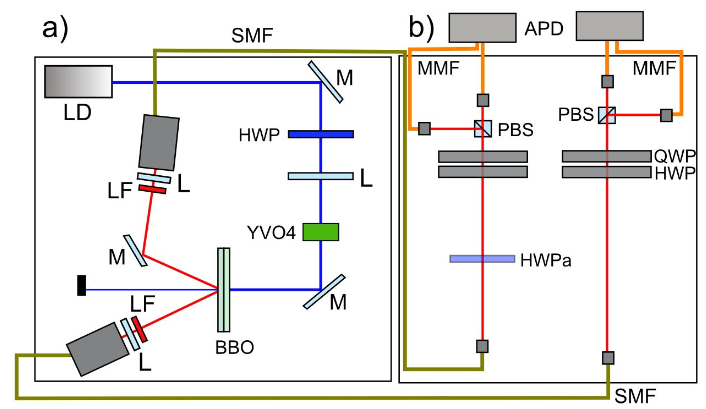
\includegraphics[scale = 0.8]{figures/setup.png}
    \caption{Schematic setup of the experiment:  laser diode (LD), longpass filter (LF), half-wave plate (HWP), lens
(L), Yttrium orthovanadate compensation crystal (YVO4), mirror (M), SPDC beta barium borate crystal (BBO), single-mode fiber
(SMF), additional half-wave plate (HWPa), polarization beam splitter (PBS), multi-
mode fiber (MMF),avalanche photodiode single photon detectors (APD).}
    \label{fig:setup}
\end{figure}


\subsection{Generation of Entangled Photons}

In order to generate entangled photon pairs we levy an optical process called Spontaneous Parametric Down-Conversion (SPDC). The SPDC process is the annihilation of a pump (p) photon into the creation of two photon signal(s) and idler(i), while conserving energy and momentum in a non-linear medium which is called the phase matching conditions, Figure \ref{fig:spdc}. The phase matching conditions can be classified in difference polarizations of the photons, if the three photons shave the same polarization, the SPDC is of type 0; if the signal and idler photons have the same polarization but are orthogonal to the pump polarization, it is of type I; if the signal and idler photons have perpendicular polarizations, it is of type II \cite{zhang2021spdc}. Momentum conservation implies that the two down converted photons are emitted in symmetric cones as in Figure \ref{fig:bbo}

In the experiment the pump beam consists of a blue laser diode (labeled LD in Figure \ref{fig:setup}) with vertical polarization (V) and wavelength 404 nm. Two type-1 nonlinear crystals of Beta-barium Borate (BBO) which are optically contacted with perpendicular optical axes, Fig. \ref{fig:bbo}, such that when illuminated by +45\textdegree polarized light (equal compositions of H and V) there is equal chance that a pump photon is converted in either of the crystals. In order to polarize the pump beam to 45\textdegree, a half wave plate is used to convert the vertically polarized blue laser diode (blue HWP in Figure \ref{fig:setup} a)).

\begin{figure}[htp]
    \centering
    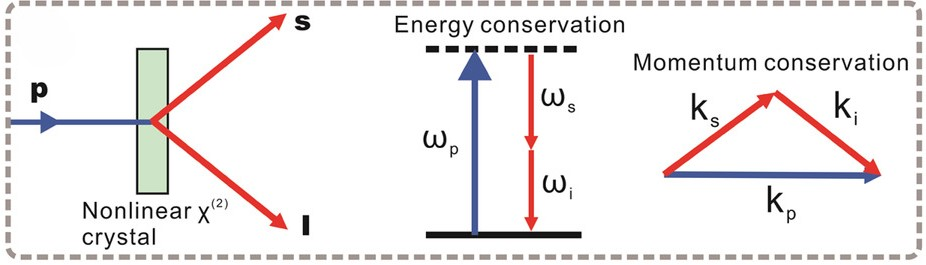
\includegraphics[scale = 4]{figures/spdc.jpg}
    \caption{Schematic of SPDC process \cite{zhang2021spdc}.}.
    \label{fig:spdc}
\end{figure} 

However, as seen in Figure \ref{fig:bbo}, H and V polarized photons have a different optical path length, and can be distinguished by their detection time. Ideally, the cones in Figure \ref{fig:bbo} should perfectly align. To account for this difference, a Yttrium vanadate crystal is placed on the beam path (YV04 in Figure \ref{fig:setup}). By tilting the crystal a phase between the H and V polarizations can be created such that H and V down-converted photons have no temporal separation. In the end we produce the state:

\begin{equation}
\begin{aligned}
|\phi\rangle &= |H, A, E_1\rangle \otimes |H, B, E_2\rangle 
+ e^{i\phi} |V, A, E_1\rangle \otimes |V, B, E_2\rangle \\
&= |A, B\rangle \otimes |E_1, E_2\rangle \big(|HH\rangle + e^{i\phi} |VV\rangle \big)
\end{aligned}
\label{eq:bell_state}
\end{equation}

where A and B are the two spatially selected modes and $E_1$ and $E_2$ are their energies. In the next subsection,, the polarization analysis of the entangled photon pairs and how to produce other Bell states are explained.


\begin{figure}[htp]
    \centering
    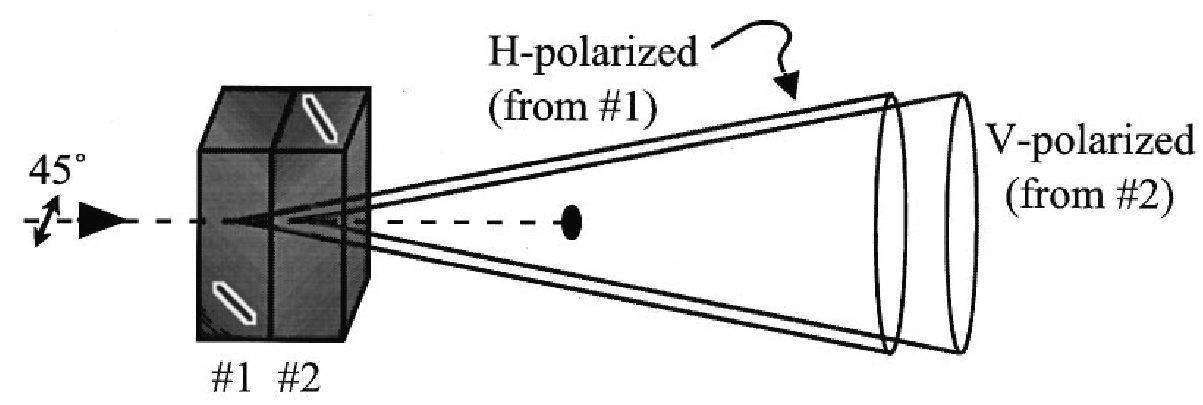
\includegraphics[scale = 0.6]{figures/bbo.png}
    \caption{Two BBO crystals we use in the experiment and the production of H and V polarized photons when illuminated with a diagonally polarized light \cite{manual}.}
    \label{fig:bbo}
\end{figure} 

\newpage

\subsection{Measurement System}
\label{subsec:measurement_system}
\begin{figure}[htp]
    \centering
    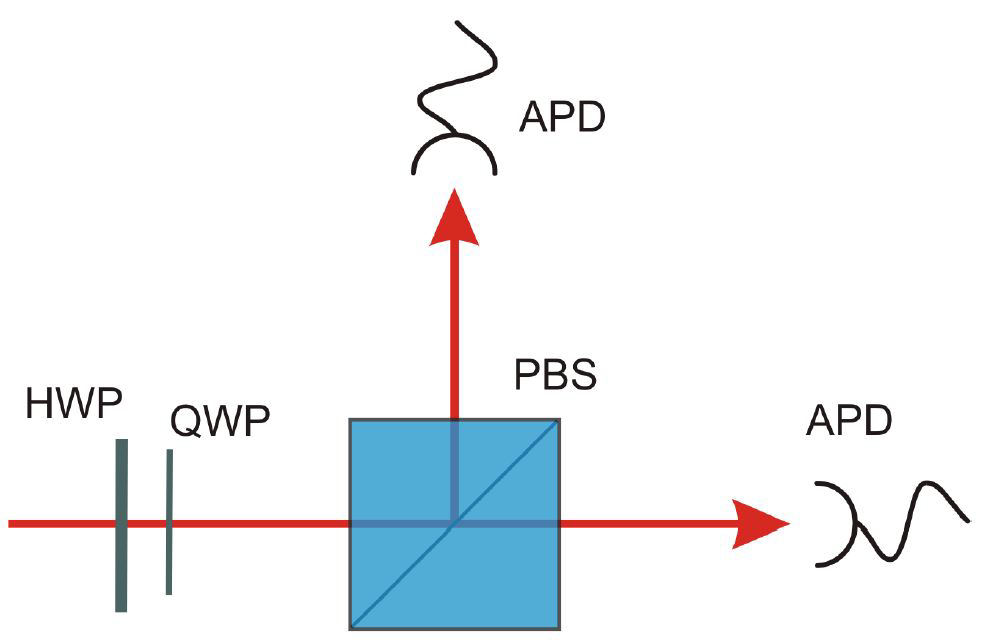
\includegraphics[scale = 0.6]{figures/apd.png}
    \caption{Polarization analysis setup for one of the arms \cite{manual}. PBS: Polarizing Beam Splitter, HWP: Half-wave plate, QWP: Quarter-wave plate, APD: Avalanche photodiode.}
    \label{fig:apd}
\end{figure} 
A polarizing beam splitter (PBS) is used to make measurements. The PBS transmits H polarized light and reflects V polarized light. Without using any wave-plates, the PBS allows us to measure polarization of the photons in the H/V basis. To measure the polarizations in other directions (left/right hand polarized or $+$/$-$) we use half-waveplates (HWP) and quarter-waveplates (QWP) to project those directions onto the H/V basis. For example from R to H we need a QWP with 45 degrees (HWP 0) and from $+$ to H we need a HWP with 22.5 degrees (QWP 0). The action of the waveplates are as follows (the angles are defined relative to the H axis) :

\begin{equation}
\hat{\sigma}_z = \text{QWP}(\alpha_{\text{QWP}}) \, \text{HWP}(\alpha_{\text{HWP}}) \, \hat{\sigma}_{\theta,\phi} \, \text{HWP}^\dagger(\alpha_{\text{HWP}}) \, \text{QWP}^\dagger(\alpha_{\text{QWP}}),
\label{eq:2.5}
\end{equation}

\begin{equation}
\text{HWP}(\alpha_{\text{HWP}}) =
\begin{pmatrix}
\cos(2\alpha_{\text{HWP}}) & \sin(2\alpha_{\text{HWP}}) \\
\sin(2\alpha_{\text{HWP}}) & -\cos(2\alpha_{\text{HWP}})
\end{pmatrix}.
\end{equation}

\begin{equation}
\text{QWP}(\alpha_{\text{QWP}}) =
\begin{pmatrix}
\cos^2(\alpha_{\text{QWP}}) - i\sin^2(\alpha_{\text{QWP}}) & (1 + i)\cos(\alpha_{\text{QWP}})\sin(\alpha_{\text{QWP}}) \\
(1 + i)\cos(\alpha_{\text{QWP}})\sin(\alpha_{\text{QWP}}) & -i\cos^2(\alpha_{\text{QWP}}) + \sin^2(\alpha_{\text{QWP}})
\end{pmatrix}.
\end{equation}
\hyperref[tab:waveplate_settings]{Table \ref*{tab:waveplate_settings}} shows the required angles of the waveplates to check correlations in different basis, X,Y,Z correspond to $+$/$-$, R/L, H/V basis respectively. Each entangled photon pair gets detected in 2 detectors in the basis HH,HV,VH and VV which is a coincidence event, that are used to construct the density matrix of the photon pair.



\begin{table}[h!]
\centering
\begin{tabular}{|c|c|c|c|c|c|}
\hline
\multicolumn{2}{|c|}{\textbf{}} & \textbf{HWP A} & \textbf{QWP A} & \textbf{HWP B} & \textbf{QWP B} \\ \hline
X              & X                     & 22.5           & 0              & 22.5           & 0              \\ \hline
X              & Y                     & 22.5           & 0              & 0              & 45             \\ \hline
X              & Z                     & 22.5           & 0              & 0              & 0              \\ \hline
Y              & X                     & 0              & 45             & 22.5           & 0              \\ \hline
Y              & Y                     & 0              & 45             & 0              & 45             \\ \hline
Y              & Z                     & 0              & 45             & 0              & 0              \\ \hline
Z              & X                     & 0              & 0              & 22.5           & 0              \\ \hline
Z              & Y                     & 0              & 0              & 0              & 45             \\ \hline
Z              & Z                     & 0              & 0              & 0              & 0              \\ \hline
\end{tabular}
\caption{Waveplate settings for quantum state tomography of $|\phi^+\rangle$.}
\label{tab:waveplate_settings}
\end{table}
We also use an additional waveplate on one of the arms to produce other Bell states from $|\phi^+\rangle$. 
To rotate the Bell state \( |\phi^+\rangle = \frac{1}{\sqrt{2}} (|HH\rangle + |VV\rangle) \) into the other Bell states:
 \( |\phi^-\rangle = \frac{1}{\sqrt{2}} (|HH\rangle - |VV\rangle) \) can be achieved by placing a Half-Wave Plate (HWP) at \( 0^\circ \) to introduce a \( \pi \)-phase shift.
 \( |\psi^+\rangle = \frac{1}{\sqrt{2}} (|HV\rangle + |VH\rangle) \) can be obtained by placing a HWP at \( 45^\circ \) to swap \(|H\rangle\) and \(|V\rangle\).
 \( |\psi^-\rangle = \frac{1}{\sqrt{2}} (|HV\rangle - |VH\rangle) \) requires both a HWP at \( 45^\circ \) and a Quarter-Wave Plate (QWP) at \( 90^\circ \) for phase adjustment.